% Template for thesis format at Department of Psychology, Senshu University
\documentclass[12pt,a4paper,xelatex,ja=standard]{bxjsarticle}
\geometry{left = 3.5cm, right = 3.5cm, top = 4.5cm, bottom = 4.5cm}
\renewcommand{\figurename}{Figure}
\renewcommand{\tablename}{Table}

\usepackage{lmodern}
\usepackage{amssymb,amsmath}
\usepackage{ifxetex,ifluatex}
\ifnum 0\ifxetex 1\fi\ifluatex 1\fi=0 % if pdftex
  \usepackage[T1]{fontenc}
  \usepackage[utf8]{inputenc}
  \usepackage{textcomp} % provide euro and other symbols
\else % if luatex or xetex
  \usepackage{unicode-math}
  \defaultfontfeatures{Scale=MatchLowercase}
  \defaultfontfeatures[\rmfamily]{Ligatures=TeX,Scale=1}
\fi
% Use upquote if available, for straight quotes in verbatim environments
\IfFileExists{upquote.sty}{\usepackage{upquote}}{}
\IfFileExists{microtype.sty}{% use microtype if available
  \usepackage[]{microtype}
  \UseMicrotypeSet[protrusion]{basicmath} % disable protrusion for tt fonts
}{}
\makeatletter
\@ifundefined{KOMAClassName}{% if non-KOMA class
  \IfFileExists{parskip.sty}{%
    \usepackage{parskip}
  }{% else
    \setlength{\parindent}{0pt}
    \setlength{\parskip}{6pt plus 2pt minus 1pt}}
}{% if KOMA class
  \KOMAoptions{parskip=half}}
\makeatother
\usepackage{xcolor}
\IfFileExists{xurl.sty}{\usepackage{xurl}}{} % add URL line breaks if available
\IfFileExists{bookmark.sty}{\usepackage{bookmark}}{\usepackage{hyperref}}
\hypersetup{
  pdftitle={こんにちは:},
  pdfauthor={学籍番号:202430325 氏名:八斗啓悟},
  hidelinks,
  pdfcreator={LaTeX via pandoc}}
\urlstyle{same} % disable monospaced font for URLs
\usepackage{color}
\usepackage{fancyvrb}
\newcommand{\VerbBar}{|}
\newcommand{\VERB}{\Verb[commandchars=\\\{\}]}
\DefineVerbatimEnvironment{Highlighting}{Verbatim}{commandchars=\\\{\}}
% Add ',fontsize=\small' for more characters per line
\usepackage{framed}
\definecolor{shadecolor}{RGB}{248,248,248}
\newenvironment{Shaded}{\begin{snugshade}}{\end{snugshade}}
\newcommand{\AlertTok}[1]{\textcolor[rgb]{0.94,0.16,0.16}{#1}}
\newcommand{\AnnotationTok}[1]{\textcolor[rgb]{0.56,0.35,0.01}{\textbf{\textit{#1}}}}
\newcommand{\AttributeTok}[1]{\textcolor[rgb]{0.13,0.29,0.53}{#1}}
\newcommand{\BaseNTok}[1]{\textcolor[rgb]{0.00,0.00,0.81}{#1}}
\newcommand{\BuiltInTok}[1]{#1}
\newcommand{\CharTok}[1]{\textcolor[rgb]{0.31,0.60,0.02}{#1}}
\newcommand{\CommentTok}[1]{\textcolor[rgb]{0.56,0.35,0.01}{\textit{#1}}}
\newcommand{\CommentVarTok}[1]{\textcolor[rgb]{0.56,0.35,0.01}{\textbf{\textit{#1}}}}
\newcommand{\ConstantTok}[1]{\textcolor[rgb]{0.56,0.35,0.01}{#1}}
\newcommand{\ControlFlowTok}[1]{\textcolor[rgb]{0.13,0.29,0.53}{\textbf{#1}}}
\newcommand{\DataTypeTok}[1]{\textcolor[rgb]{0.13,0.29,0.53}{#1}}
\newcommand{\DecValTok}[1]{\textcolor[rgb]{0.00,0.00,0.81}{#1}}
\newcommand{\DocumentationTok}[1]{\textcolor[rgb]{0.56,0.35,0.01}{\textbf{\textit{#1}}}}
\newcommand{\ErrorTok}[1]{\textcolor[rgb]{0.64,0.00,0.00}{\textbf{#1}}}
\newcommand{\ExtensionTok}[1]{#1}
\newcommand{\FloatTok}[1]{\textcolor[rgb]{0.00,0.00,0.81}{#1}}
\newcommand{\FunctionTok}[1]{\textcolor[rgb]{0.13,0.29,0.53}{\textbf{#1}}}
\newcommand{\ImportTok}[1]{#1}
\newcommand{\InformationTok}[1]{\textcolor[rgb]{0.56,0.35,0.01}{\textbf{\textit{#1}}}}
\newcommand{\KeywordTok}[1]{\textcolor[rgb]{0.13,0.29,0.53}{\textbf{#1}}}
\newcommand{\NormalTok}[1]{#1}
\newcommand{\OperatorTok}[1]{\textcolor[rgb]{0.81,0.36,0.00}{\textbf{#1}}}
\newcommand{\OtherTok}[1]{\textcolor[rgb]{0.56,0.35,0.01}{#1}}
\newcommand{\PreprocessorTok}[1]{\textcolor[rgb]{0.56,0.35,0.01}{\textit{#1}}}
\newcommand{\RegionMarkerTok}[1]{#1}
\newcommand{\SpecialCharTok}[1]{\textcolor[rgb]{0.81,0.36,0.00}{\textbf{#1}}}
\newcommand{\SpecialStringTok}[1]{\textcolor[rgb]{0.31,0.60,0.02}{#1}}
\newcommand{\StringTok}[1]{\textcolor[rgb]{0.31,0.60,0.02}{#1}}
\newcommand{\VariableTok}[1]{\textcolor[rgb]{0.00,0.00,0.00}{#1}}
\newcommand{\VerbatimStringTok}[1]{\textcolor[rgb]{0.31,0.60,0.02}{#1}}
\newcommand{\WarningTok}[1]{\textcolor[rgb]{0.56,0.35,0.01}{\textbf{\textit{#1}}}}
\usepackage{graphicx}
\makeatletter
\def\maxwidth{\ifdim\Gin@nat@width>\linewidth\linewidth\else\Gin@nat@width\fi}
\def\maxheight{\ifdim\Gin@nat@height>\textheight\textheight\else\Gin@nat@height\fi}
\makeatother
% Scale images if necessary, so that they will not overflow the page
% margins by default, and it is still possible to overwrite the defaults
% using explicit options in \includegraphics[width, height, ...]{}
\setkeys{Gin}{width=\maxwidth,height=\maxheight,keepaspectratio}
% Set default figure placement to htbp
\makeatletter
\def\fps@figure{htbp}
\makeatother
\setlength{\emergencystretch}{3em} % prevent overfull lines
\providecommand{\tightlist}{%
  \setlength{\itemsep}{0pt}\setlength{\parskip}{0pt}}
\setcounter{secnumdepth}{-\maxdimen} % remove section numbering

\title{こんにちは:}
\author{学籍番号:202430325 氏名:八斗啓悟}
\date{}
\usepackage{marginnote}
\usepackage{titlesec}
\titleformat{\section}[hang]{\large\filcenter\bfseries}{\thesection}{1zw}{}

\usepackage{booktabs}
\usepackage{longtable}
\usepackage{array}
\usepackage{multirow}
\usepackage{wrapfig}
\usepackage{float}
\usepackage{colortbl}
\usepackage{pdflscape}
\usepackage{tabu}
\usepackage{threeparttable}
\usepackage{threeparttablex}
\usepackage[normalem]{ulem}
\usepackage{makecell}
\usepackage{xcolor}
\usepackage{graphicx}

\begin{document}
\pagestyle{empty}
\maketitle
\clearpage
{
\setcounter{tocdepth}{3}
\tableofcontents
}
\clearpage
\pagestyle{plain}
\setcounter{page}{1}

\section{序文}\label{ux5e8fux6587}

\subsection{はじめに}\label{ux306fux3058ux3081ux306b}

まず,Kunisato et al.(2012)
のように,すると,bibファイル内のKunisatoの2012年の論文が引用されます。そして,次のように,{[}{]}でくくると文末の引用スタイルになります(国里他,
2019)。また,文末に複数引用する場合は,こういう感じにします(国里他,
2019; Machino et al., 2014)。

\clearpage

01234567890123456789012345678901234567890123456789012345678901234567890123456789012345678901234567890123456789012345678901234567890123456789012345678901234567890123456789012345678901234567890123456789012345678901234567890123456789012345678901234567890123456789012345678901234567890123456789012345678901234567890123456789012345678901234567890123456789012345678901234567890123456789012345678901234567890123456789012345678901234567890123456789012345678901234567890123456789012345678901234567890123456789012345678901234567890123456789012345678901234567890123456789012345678901234567890123456789012345678901234567890123456789012345678901234567890123456789012345678901234567890123456789012345678901234567890123456789012345678901234567890123456789012345678901234567890123456789012345678901234567890123456789ここから八百字超えています。

\subsection{先行研究について}\label{ux5148ux884cux7814ux7a76ux306bux3064ux3044ux3066}

\subsubsection{先行研究での知見1}\label{ux5148ux884cux7814ux7a76ux3067ux306eux77e5ux898buxff11}

\subsubsection{先行研究での知見2}\label{ux5148ux884cux7814ux7a76ux3067ux306eux77e5ux898b2}

\subsubsection{先行研究での知見3}\label{ux5148ux884cux7814ux7a76ux3067ux306eux77e5ux898b3}

\subsubsection{先行研究での知見4}\label{ux5148ux884cux7814ux7a76ux3067ux306eux77e5ux898b4}

\subsubsection{先行研究での知見5}\label{ux5148ux884cux7814ux7a76ux3067ux306eux77e5ux898b5}

\subsubsection{先行研究での知見6}\label{ux5148ux884cux7814ux7a76ux3067ux306eux77e5ux898buxff16}

\subsubsection{先行研究での知見7}\label{ux5148ux884cux7814ux7a76ux3067ux306eux77e5ux898buxff17}

\subsection{先行研究の問題点}\label{ux5148ux884cux7814ux7a76ux306eux554fux984cux70b9}

\section{目的}\label{ux76eeux7684}

\clearpage

\section{方法}\label{ux65b9ux6cd5}

\subsection{実験or調査参加者}\label{ux5b9fux9a13orux8abfux67fbux53c2ux52a0ux8005}

神奈川県内の私立大学生2800名(男性919名,女性1881名)が実験or調査に参加した。参加者の平均年齢
(標準偏差) は,28.78歳(11.13)であった。

\subsection{行動課題や質問紙}\label{ux884cux52d5ux8ab2ux984cux3084ux8ceaux554fux7d19}

\subsection{実験手続き(調査手続き)}\label{ux5b9fux9a13ux624bux7d9aux304dux8abfux67fbux624bux7d9aux304d}

\subsection{統計解析}\label{ux7d71ux8a08ux89e3ux6790}

 統計解析は,Windows 11 x64 (build 22631)上で,R version 4.4.1
(2024-06-14
ucrt)を用いて実施された。使用されたRパッケージは以下の通りになる。

\begin{table}[!h]
\centering
\caption{\label{tab:unnamed-chunk-3}使用Rパッケージ}
\centering
\begin{tabular}[t]{ll}
\toprule
R packages & Version\\
\midrule
\cellcolor{gray!10}{dplyr} & \cellcolor{gray!10}{1.1.4}\\
forcats & 1.0.0\\
\cellcolor{gray!10}{ggplot2} & \cellcolor{gray!10}{3.5.1}\\
ggsignif & 0.6.4\\
\cellcolor{gray!10}{gridExtra} & \cellcolor{gray!10}{2.3}\\
\addlinespace
jtools & 2.3.0\\
\cellcolor{gray!10}{kableExtra} & \cellcolor{gray!10}{1.4.0}\\
knitr & 1.49\\
\cellcolor{gray!10}{lubridate} & \cellcolor{gray!10}{1.9.3}\\
psych & 2.4.6.26\\
\addlinespace
\cellcolor{gray!10}{purrr} & \cellcolor{gray!10}{1.0.2}\\
readr & 2.1.5\\
\cellcolor{gray!10}{stringr} & \cellcolor{gray!10}{1.5.1}\\
tibble & 3.2.1\\
\cellcolor{gray!10}{tidyr} & \cellcolor{gray!10}{1.3.1}\\
\addlinespace
tidyverse & 2.0.0\\
\bottomrule
\end{tabular}
\end{table}

\clearpage

\section{結果}\label{ux7d50ux679c}

\subsection{記述統計}\label{ux8a18ux8ff0ux7d71ux8a08}

\begin{table}[!h]
\centering
\caption{\label{tab:unnamed-chunk-4}Descriptive Statistics of bfi}
\centering
\begin{tabular}[t]{rrrrrrrr}
\toprule
n & Mean & SD & Median & Min & Max & Skewness & kurtosis\\
\midrule
\cellcolor{gray!10}{2713} & \cellcolor{gray!10}{18.96} & \cellcolor{gray!10}{2.71} & \cellcolor{gray!10}{19} & \cellcolor{gray!10}{5} & \cellcolor{gray!10}{29} & \cellcolor{gray!10}{0.01} & \cellcolor{gray!10}{1.08}\\
2694 & 15.82 & 5.97 & 15 & 5 & 30 & 0.22 & -0.66\\
\cellcolor{gray!10}{2707} & \cellcolor{gray!10}{19.04} & \cellcolor{gray!10}{2.77} & \cellcolor{gray!10}{19} & \cellcolor{gray!10}{5} & \cellcolor{gray!10}{30} & \cellcolor{gray!10}{-0.17} & \cellcolor{gray!10}{0.81}\\
2709 & 21.04 & 3.68 & 22 & 5 & 30 & -0.66 & 0.68\\
\cellcolor{gray!10}{2726} & \cellcolor{gray!10}{19.34} & \cellcolor{gray!10}{2.74} & \cellcolor{gray!10}{19} & \cellcolor{gray!10}{5} & \cellcolor{gray!10}{29} & \cellcolor{gray!10}{-0.02} & \cellcolor{gray!10}{1.09}\\
\bottomrule
\end{tabular}
\end{table}

\begin{center}
Note. SD=standard deviation
\end{center}

\subsection{メインの解析の前提となる解析}\label{ux30e1ux30a4ux30f3ux306eux89e3ux6790ux306eux524dux63d0ux3068ux306aux308bux89e3ux6790}

\begin{figure}
\centering
\includegraphics{fig1.png}
\caption{How R Markdown works}
\end{figure}

\begin{figure}[H]
\centering
\includegraphics[clip,width = 8cm]{fig1.png}
\caption{How R Markdown works}    
\end{figure}

\subsection{メインの解析の記載}\label{ux30e1ux30a4ux30f3ux306eux89e3ux6790ux306eux8a18ux8f09}

\begin{figure}
\centering
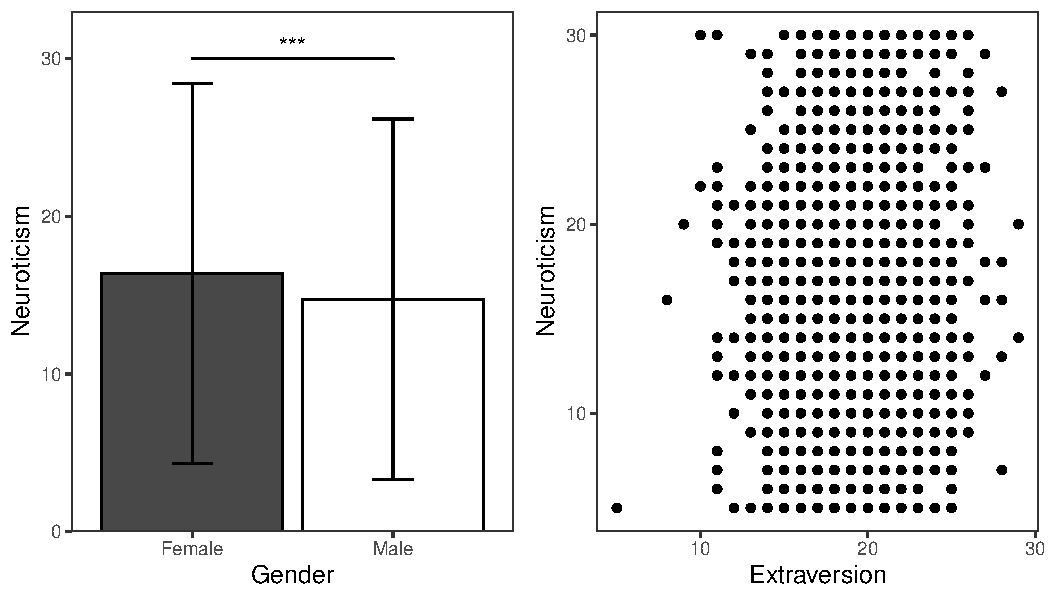
\includegraphics{paper_files/figure-latex/figs-1.pdf}
\caption{\label{fig:figs}Examples of bar plot and scatter plot}
\end{figure}

\subsection{メインの解析結果を補強する解析の記載}\label{ux30e1ux30a4ux30f3ux306eux89e3ux6790ux7d50ux679cux3092ux88dcux5f37ux3059ux308bux89e3ux6790ux306eux8a18ux8f09}

\clearpage

\section{考察}\label{ux8003ux5bdf}

\subsection{主要な発見の概要}\label{ux4e3bux8981ux306aux767aux898bux306eux6982ux8981}

\subsection{考えられるメカニズムの考察と説明}\label{ux8003ux3048ux3089ux308cux308bux30e1ux30abux30cbux30baux30e0ux306eux8003ux5bdfux3068ux8aacux660e}

\subsection{関連のある先行研究の結果との比較}\label{ux95a2ux9023ux306eux3042ux308bux5148ux884cux7814ux7a76ux306eux7d50ux679cux3068ux306eux6bd4ux8f03}

\subsection{研究結果が与える示唆}\label{ux7814ux7a76ux7d50ux679cux304cux4e0eux3048ux308bux793aux5506}

\subsection{研究の限界と今後の課題}\label{ux7814ux7a76ux306eux9650ux754cux3068ux4ecaux5f8cux306eux8ab2ux984c}

\subsection{結論}\label{ux7d50ux8ad6}

\clearpage

\section{要約}\label{ux8981ux7d04}

\clearpage

\section{引用文献}\label{ux5f15ux7528ux6587ux732e}

\noindent \begingroup \setlength{\parindent}{-0.3in}
\setlength{\leftskip}{0.2in} \setlength{\parskip}{8pt}

国里~愛彦・片平~健太郎・沖村~宰・山下~祐一 (2019).
うつに対する計算論的アプローチ:―強化学習モデルの観点から― ~ 心理学評論,
\emph{62}(1), 88-103.~\verb|10.24602/sjpr.62.1_88|

Kunisato, Y. , Okamoto, Y. , Ueda, K. , Onoda, K. , Okada, G. ,
Yoshimura, S. \ldots Yamawaki, S. (2012). Effects of depression on
reward-based decision making and variability of action in probabilistic
learning,
\emph{Journal of behavior therapy and experimental psychiatry},
\emph{43}(4), 1088--1094.

Machino, A. , Kunisato, Y. , Matsumoto, T. , Yoshimura, S. , Ueda, K. ,
Yamawaki, Y. \ldots Yamawaki, S. (2014). Possible involvement of
rumination in gray matter abnormalities in persistent symptoms of major
depression: an exploratory magnetic resonance imaging voxel-based
morphometry study, \emph{Journal of affective disorders}, \emph{168},
229--235.

\endgroup

\clearpage

\section{謝辞}\label{ux8b1dux8f9e}

\clearpage

\section{付録}\label{ux4ed8ux9332}

\begin{Shaded}
\begin{Highlighting}[]
\FunctionTok{library}\NormalTok{(tidyverse)}
\end{Highlighting}
\end{Shaded}


\end{document}
